\documentclass[10pt]{article}

%\usepackage{titling}
\usepackage[utf8]{inputenc}
%\usepackage[ngerman]{babel}
\usepackage{scrpage2}
\usepackage{graphicx}
%\usepackage{lastpage}
%\usepackage[a4paper,left=2.5cm,right=2cm,top=1cm,bottom=2.5cm]{geometry}
\usepackage{float}
%\renewcommand*\familydefault{\sfdefault} 
\usepackage[T1]{fontenc}
%\usepackage{booktabs}
%\usepackage{pdflscape}
\usepackage[table,xcdraw]{xcolor}

\renewcommand{\headfont}{}

\usepackage{hyperref}



\usepackage[square,numbers]{natbib} 
\bibliographystyle{plainnat}

\title{Software Requirement Specification}
\date{13.12.2016}
\author{\textbf{ESE Team 9} \\ \\Sven Kellenberger\\Rafael
Ottersberg\\Levi Ryffel\\Marcel Schmutz\\Kevin Studer}




%\pagestyle{scrheadings}
%\ihead{Test}
%\ohead{Test}
%\ofoot{Test}



\begin{document}
\maketitle
\pagebreak
\tableofcontents
\pagebreak

\section{Introduction}

\subsection{Purpose}
This document presents a detailed description of the web application Flatfindr.
Foremost, it provides a legaly binding contract between the stakeholders and the
developer team 9. This document is a RUP conform SRS document.

\subsection{Scope of the Project}
The web application Flatfindr will help the participating user to promote free
places in their houses or flats. Also it should help user to search for free
places in houses or flats.

More specifically, the application will provide methods to search for free
flats, help to ensure flats with specific parameters are presented for users and
that the application will provide enough methods, to get in contact with the
advertiser. On the other side, users will be able to insert an ad for a free
place in their flats, will help define the visitation time (if an user wants to
see the flat which is advertised) and provide some other instruments to describe
the flat as best as possible.

\subsection{Glossary}

\begin{table}[H]
	\centering
	\begin{tabular}{p{3cm}p{9cm}}
	\multicolumn{1}{c}{\textbf{Term}} & \multicolumn{1}{c}{\textbf{Description}} \\
Advertiser & User who advertise his free place in his house or flat. \\
RUP & Stands for Rational Unified Process. Process developed by IBM. Has the SRS document as a requirement for all development activities. \\
SRS & Stands for Software Requirements Specification. A document that completely describes all of the functions of a proposed system and the constraints under which it must operate. \\
Stakeholder & Any person with an interest in the project who is not a developer. \\
User & Participant in the application. Can either be a normal user who searches for a flat or an advertiser. 
	\end{tabular}
	\caption{Glossary}
	\label{table-glossary}
\end{table}

\subsection{Stakeholders}
The table \ref{table-stakeholders} will give an overview of the known
Stakeholders.
\begin{table}[H]
	\centering
	\begin{tabular}{ll}
	\multicolumn{1}{c}{\textbf{Name}} & \multicolumn{1}{c}{\textbf{Contact}} \\
	ESE Assistant & ?                                        
	\end{tabular}
	\caption{Stakeholders}
	\label{table-stakeholders}
\end{table}
%TODO: Identify Stakeholders

\subsection{System Overview}
The image \ref{image-system-overview} will introduce a general system overview
of the product in development.
\begin{figure}[p]
    \centering
	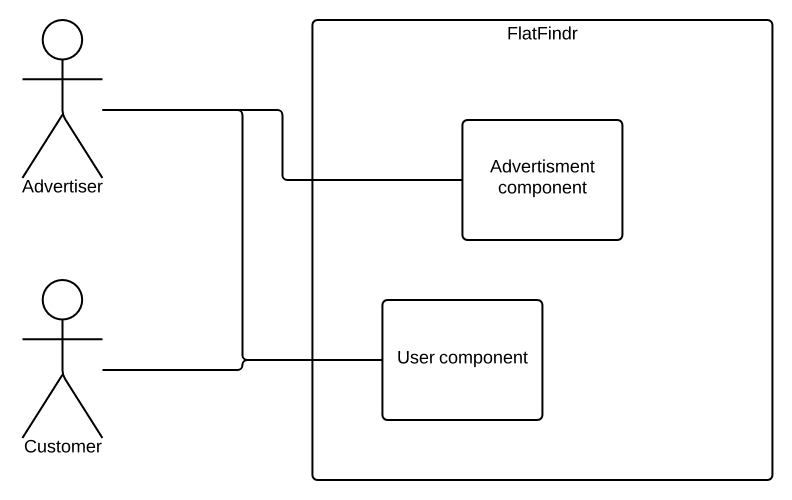
\includegraphics[width=12cm]{images/system-overview}
	\caption{System Overview}
    \label{image-system-overview}
\end{figure}

\subsection{References}

\section{Overall Description}
\subsection{Product Perspective}
	Flatfindr is a self-contained product that has no connections to other software.	

\subsection{Product Functions}
\begin{itemize}
	\item Creating / viewing ads for flats and flats
	\item Linking housemates to ads
	\item General search functionality with specific criteria
	\item Scheduling visits
	\end{itemize}

\subsection{User Classes and Characteristics}
	\subsubsection{User}
		The general user has two main roles which are not necessarily mutually exclusive. These are: \\
		\begin{enumerate}
		\item 		Advertiser: A user can place an ad (for free) on the homepage, which is then publicly visible.
		\item		Client: A client can look through the ads put up by advertisers and can contact the advertisers via the message functionality.
		\end{enumerate}
		
	\subsubsection{Premium User}
		By paying a fee for additional features, the premium user strongly increases the resources 
		of the programming team. If the premium features are beneficial to the general user, the 
		quantity of premium users will be optimal.
		
\subsection{Operating Environment}
	Flatfindr runs on any frequently used browser, i.e. Firefox, Safari, Chrome, Microsoft Edge, Internet Explorer.
	
\subsection{Design and Implementation Constraints}
	The template of Flatfindr was delivered using Java, MySQL, Hibernation and JavaScript. Changing this would 
	present unnecessary additional effort, which is why, in this way, we are constrained by these frameworks and languages.\\
	The software should be maintainable, so object-oriented design will be best-practice.
	Other than that, there seem to be no requirements, especially security.
\section{External Interfaces}

\subsection{User Interfaces}
	As is shown by image \ref{image-abecScreenshot}, the user interface is
	straight forward due to it being a homepage.
	
\begin{figure}[p]
    \centering
	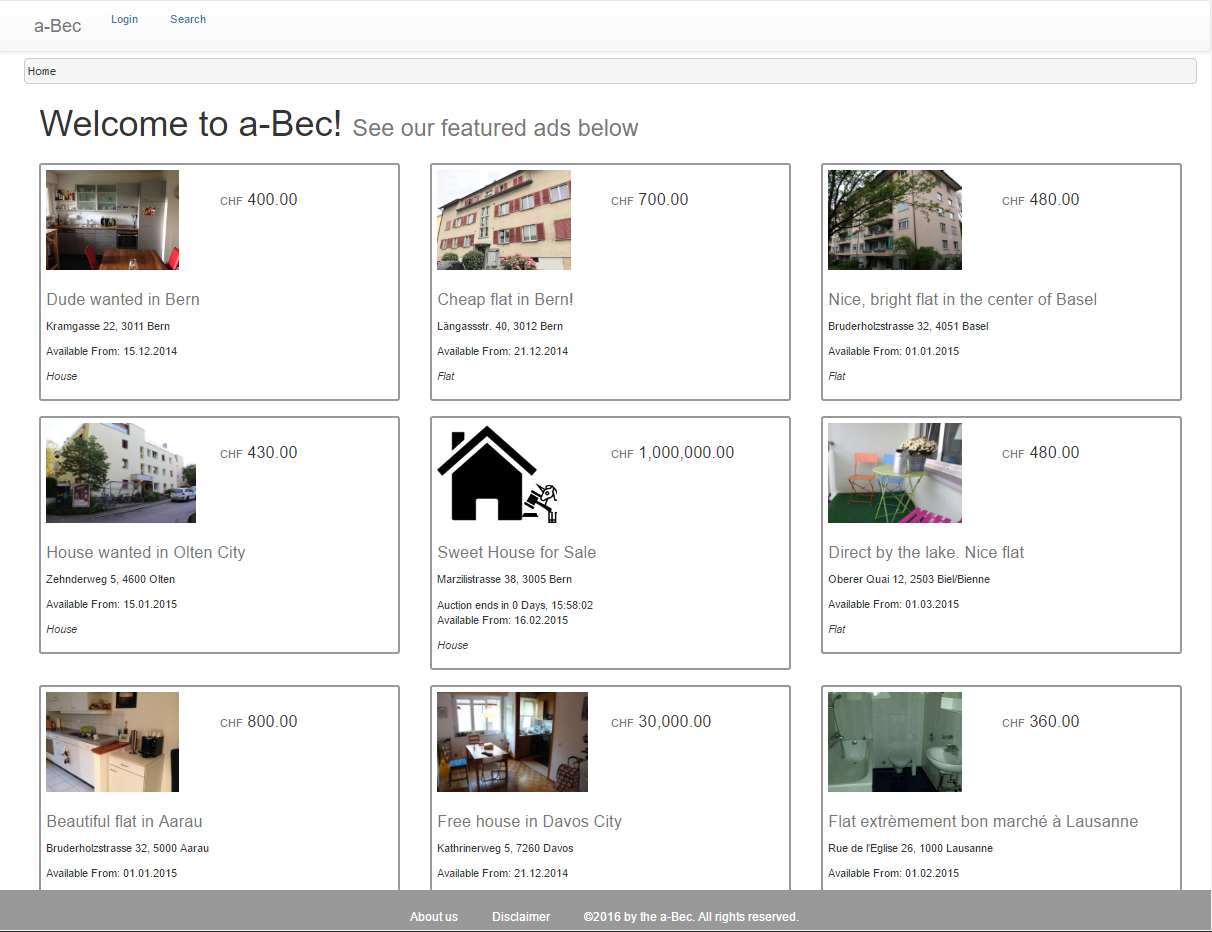
\includegraphics[width=12cm]{images/abecScreenshot}
	\caption{GUI}
    \label{image-abecScreenshot}
\end{figure}
	
\subsection{Hardware Interfaces}
	The homepage will be able to be displayed on a computer, as well as mobile
	phones and tablets.
	
\section{System Features}
\subsection{Use-Cases}
\subsubsection{User}

\begin{table}[H]
\centering
\label{table-use-case-1}
\begin{tabular}{|p{3cm}|p{10cm}}
Use Case ID       & 1                                                           
\\
Use Case Name     & Sign up                                                         
\\
Trigger           & A user wants to create a new profile
advertiser
\\
Precondition      & The user is on the login page                                                
\\
Basic Path        & \begin{enumerate}
\item The user clicks on 'sign up as a new user'
\item The user enters his information in the form
\item The use clicks the 'Sign up' button
\item The user is redirected to the login page
\end{enumerate} 
     \\
Alternative Paths & None                     
\\
Postconditions    & A new profile is created for the user
\\
Exception Paths   & If the user enters none or invalid information an error is
generated. 
\\
Other             & n/a                                                                                                                                                                                                        
\end{tabular}
\caption{Use Case 1}
\end{table}

\begin{table}[H]
\centering
\label{table-use-case-2}
\begin{tabular}{|p{3cm}|p{10cm}}
Use Case ID       & 2                                                                                                                                                              \\
Use Case Name     & Login                                                                                                                                                          \\
Trigger           & A user wants to login to the webapplication                                                                                                                   \\
Precondition      & The user has already an account on the webapplication or has a google account                                                                                                          \\
Basic Path        & \begin{enumerate}
\item The user access the webapplication and selects the link "Login"
\item The user enters his credentials for his account
\item The user is redirected to the homepage
\end{enumerate} 
     \\
Alternative Paths & The user logs in with a google account                         \\
Postconditions    & The user is logged-in                                                                                                                                          \\
Exception Paths   & In step 2, if the user enters not valid credentials into the system, the system should exit with the error message, that the credentials were wrong            \\
Other             & n/a                                                                                                                                                                                                        
\end{tabular}
\caption{Use Case 2}
\end{table}


\begin{table}[H]
\centering
\label{table-use-case-3}
\begin{tabular}{|p{3cm}|p{10cm}}
Use Case ID       & 3                                                                                                                                                              \\
Use Case Name     & Logout                                                                                                                                                         \\
Trigger           & A user wants to logout                                                                                                                   \\
Precondition      & The user is logged in                                                                                                        \\
Basic Path        & \begin{enumerate}
\item The user clicks on the link 'Logout' in the account menu
\end{enumerate} 
     \\
Alternative Paths & none                         \\
Postconditions    & The user is logged-out                                                                                                                                          \\
Exception Paths   &         \\
Other             & n/a                                                                                                                                                                                                        
\end{tabular}
\caption{Use Case 3}
\end{table}


\begin{table}[H]
\centering
\label{table-use-case-4}
\begin{tabular}{|p{3cm}|p{10cm}}
Use Case ID       & 4                                                           
\\
Use Case Name     & Edit public profile                                                        
\\
Trigger           & A user wants to edit or change his public profile
advertiser
\\
Precondition      & The user is logged in
\\
Basic Path        & \begin{enumerate}

\item The user selects 'Public profile' in the account menu
\item The user clicks on the 'Edit profile' button
\item The user changes the information he wants
\item The user clicks on the 'Update' button
\item The user is redirected to a page that says 'Your profile has been
updated!'
\end{enumerate} 
     \\
Alternative Paths & None                       
\\
Postconditions    & The information is updated on the public profile of the user and the user is logged out
\\
Exception Paths   & None                          \\
Other             & n/a                                                                                                                                                                                                        
\end{tabular}
\caption{Use Case 4}
\end{table}

\begin{table}[H]
\centering
\label{table-use-case-5}
\begin{tabular}{|p{3cm}|p{10cm}}
Use Case ID       & 5                                                         \\
Use Case Name     & Get premium                                \\
Trigger           & A user wants to be a premium user					\\
Precondition      & The user is logged in\\
Basic Path        & \begin{enumerate}
\item The user accesses the webapplication and selects the link 'Get Premium' in the user menu
\item The user is redirected to a form, where he enters the payment data.
\item After submitting the form the user is redirected to his profile page with the message 'You are now a premium user'
\end{enumerate} 
     \\
Alternative Paths & None                          \\
Postconditions    & The user is now a marvelous premium user with an unicorn next to his name.                                                          
\\
Exception Paths   & The form isn't filled in completely in step 2            \\
Other             & n/a                                                                                                                                                                                                        
\end{tabular}
\caption{Use Case 5}
\end{table}

\begin{table}[H]
\centering
\label{table-use-case-6}
\begin{tabular}{|p{3cm}|p{10cm}}
Use Case ID       & 6                                                           
\\
Use Case Name     & Message user                                                         
\\
Trigger           & A user wants to send a message to another user
\\
Precondition      & The user is logged in and on the profile page of the
receiver
\\
Basic Path        & \begin{enumerate}

\item The user clicks on the 'Message' button
\item A message form opens
\item The user types a subject
\item The user types a message
\item The user clicks on the send button
\end{enumerate} 
     \\
Alternative Paths & The client clicks on the 'Cancel' button to abort                        
\\
Postconditions    & A message is sent to the receiver
\\
Exception Paths   & None                          \\
Other             & n/a                                                                                                                                                                                                        
\end{tabular}
\caption{Use Case 6}
\end{table}

\begin{table}[H]
\centering
\label{table-use-case-7}
\begin{tabular}{|p{3cm}|p{10cm}}
Use Case ID       & 7                                                           
\\
Use Case Name     & See list of incoming/sent messages                                                         
\\
Trigger           & A user wants to see his incoming/sent messages
advertiser
\\
Precondition      & The user is logged in                                                
\\
Basic Path        & \begin{enumerate}
\item The user selects 'Messages' in the account menu
\item The user clicks on 'Inbox' to see the list of all incoming messages
\item The user clicks on a Message to see it in detail
\end{enumerate} 
     \\
Alternative Paths & The user clicks in step 2 on 'Sent' to see the list of all
sent messages
\\
Postconditions    & None
\\
Exception Paths   & None
\\
Other             & n/a                                                                                                                                                                                                        
\end{tabular}
\caption{Use Case 7}
\end{table}


\subsubsection{Client}


\begin{table}[H]
\centering
\label{table-use-case-8}
\begin{tabular}{|p{3cm}|p{10cm}}
Use Case ID       & 8                                                           
\\
Use Case Name     & See through list of ads                                                         
\\
Trigger           & A user wants to look at some ads/visits the website                                          
\\
Precondition      & None                                                 
\\
Basic Path        & \begin{enumerate}
\item The user visits the home page by entering the url or when already on the
page clicking on the 'a-Bec' logo
\end{enumerate} 
     \\
Alternative Paths & None                          \\
Postconditions    & The user is on the homepage and sees the ads                                                          
\\
Exception Paths   & None                          \\
Other             & n/a                                                                                                                                                                                                        
\end{tabular}
\caption{Use Case 8}
\end{table}


\begin{table}[H]
\centering
\label{table-use-case-9}
\begin{tabular}{|p{3cm}|p{10cm}}
Use Case ID       & 9                                                         \\
Use Case Name     & Search for ads                                                         \\
Trigger           & A user wants to look for ads                                        \\
Precondition      & The user is logged in and on the search page                             \\
Basic Path        & \begin{enumerate}
\item The user selects in the search criterias that he wants to look for
ads
\item All properties on sale (directly or through an auction) matching his other
search criterias are displayed to the user
\item The user can sort the relults by different criteria
\item The user can click on the tab 'Map' to see where the results are located
\end{enumerate} 
     \\
Alternative Paths & None                          \\
Postconditions    & None                                                      \\
Exception Paths   & None				\\
Other             & n/a                                                                                                                                                                                                        
\end{tabular}
\caption{Use Case 9}
\end{table}


\begin{table}[H]
\centering
\label{table-use-case-10}
\begin{tabular}{|p{3cm}|p{10cm}}
Use Case ID       & 10                                                           \\
Use Case Name     & Buy or rent a property                                                         \\
Trigger           & A user wants buy and rent the property described in an ad \\
Precondition      & The user is logged in and on the ad page of the property he wants to buy or rent\\
Basic Path        & \begin{enumerate}
\item The user selects the link 'Contact advertiser'
\item The user gets a form through which he can contact the seller
\end{enumerate} 
     \\
Alternative Paths & None                          \\
Postconditions    & None				\\
Exception Paths   & None            \\
Other             & n/a                                                                                                                                                                                                        
\end{tabular}
\caption{Use Case 10}
\end{table}

\begin{table}[H]
\centering
\label{table-use-case-11}
\begin{tabular}{|p{3cm}|p{10cm}}
Use Case ID       & 11                                                         \\
Use Case Name     & Bid on a property                                                          \\
Trigger           & A user wants to bid on the auction of a property                                          \\
Precondition      & The user is logged in and on an ad page with an auction                                                 \\
Basic Path        & \begin{enumerate}
\item The user can enter a bid, which has to be higher than the
present highest bid plus the minimum increment. 
\end{enumerate} 
     \\
Alternative Paths & None                          \\
Postconditions    & The highest bid now displays the bid made by the user                                                       \\
Exception Paths   & In step 3 if the bid is not higher than the present one an error flashes to point the fact out.					\\
Other             & n/a                                                                                                                                                                                                        
\end{tabular}
\caption{Use Case 11}
\end{table}


\begin{table}[H]
\centering
\label{table-use-case-12}
\begin{tabular}{|p{3cm}|p{10cm}}
Use Case ID       & 12                                                           
\\
Use Case Name     & Bookmark an ad                                                          
\\
Trigger           & A client wants to add an ad to his bookmarks                                           
\\
Precondition      & The user is logged in and the ad isn't bookmarked yet                                                 
\\
Basic Path        & \begin{enumerate}
\item The client visits an ad
\item The client presses the 'Bookmark Ad' Button
\end{enumerate} 
     \\
Alternative Paths & None                          \\
Postconditions    & The ad is added to the list 'My Bookmarks' the 'Bookmark Ad'
and Button turns to 'Bookmarked'
\\
Exception Paths   & None                          \\
Other             & n/a                                                                                                                                                                                                        
\end{tabular}
\caption{Use Case 12}
\end{table}


\begin{table}[H]
\centering
\label{table-use-case-13}
\begin{tabular}{|p{3cm}|p{10cm}}
Use Case ID       & 13                                                         \\
Use Case Name     & Create an alert                                                         \\
Trigger           & A user wants to create an alert                                         \\
Precondition      & The user is logged in                          \\
Basic Path        & \begin{enumerate}
\item The user selects the link 'Alerts' in the menu
\item The user is redirected to a form where he can select the search criterias
he want to cover with his alert
\item After submitting the form the new alert is showed in the list 'Your active alerts'
\end{enumerate} 
     \\
Alternative Paths & None                          \\
Postconditions    & The search alert is attached to the profile of the user and
he gets an email notification every time a new ad for a property matching his
alert criterias is created			\\
Exception Paths   & None				\\
Other             & n/a                                                                                                                                                                                                        
\end{tabular}
\caption{Use Case 13}
\end{table}


\begin{table}[H]
\centering
\label{table-use-case-14}
\begin{tabular}{|p{3cm}|p{10cm}}
Use Case ID       & 14                                                         \\
Use Case Name     & Delete an alert                                      \\
Trigger           & A user wants to delete a previously created alert	\\
Precondition      & The user is logged in and on his profile page               \\
Basic Path        & \begin{enumerate}
\item The user selects the link 'Alerts' in the menu
\item The user is redirected to the search alerts page, where all his search
alerts are displayed. He can now delete each alert with the 'delete' buttons
\end{enumerate} 
     \\
Alternative Paths & None                          \\
Postconditions    & The user gets no longer notifications for deleted alerts and they dissapear from the active alerts list    \\
Exception Paths   & None			\\
Other             & n/a                                                                                                                                                                                                        
\end{tabular}
\caption{Use Case 14}
\end{table}


\begin{table}[H]
\centering
\label{table-use-case-15}
\begin{tabular}{|p{3cm}|p{10cm}}
Use Case ID       & 15                                                           
\\
Use Case Name     & See list of bookmarked ads                                                         
\\
Trigger           & A client wants to look at all his bookmarked ads                                          
\\
Precondition      & The user is logged in                                                
\\
Basic Path        & \begin{enumerate}
\item The client selects 'My bookmarks' in the account menu
\end{enumerate} 
     \\
Alternative Paths & None                          \\
Postconditions    & The list 'My Bookmarks' is presented
\\
Exception Paths   & None                          \\
Other             & n/a                                                                                                                                                                                                        
\end{tabular}
\caption{Use Case 15}
\end{table}


\begin{table}[H]
\centering
\label{table-use-case-16}
\begin{tabular}{|p{3cm}|p{10cm}}
Use Case ID       & 16                                                           
\\
Use Case Name     & See a list of all auctions you participated in                                                         
\\
Trigger           & A client wants to look at all auctions he participated in                                          
\\
Precondition      & The user is logged in                                                
\\
Basic Path        & \begin{enumerate}
\item The client selects 'My participated auctions' in the account menu
\end{enumerate} 
     \\
Alternative Paths & None                          \\
Postconditions    & The list 'My participated auctions' is presented with the most important information for every auction
\\
Exception Paths   & None                          \\
Other             & n/a                                                                                                                                                                                                        
\end{tabular}
\caption{Use Case 16}
\end{table}


\subsubsection{Advertiser}


\begin{table}[H]
\centering
\label{table-use-case-17}
\begin{tabular}{|p{3cm}|p{10cm}}
Use Case ID       & 17                                                        \\
Use Case Name     & Place a renting ad                            \\
Trigger           & A user wants to place a renting ad\\
Precondition      & The user is logged in             \\
Basic Path        & \begin{enumerate}
\item The user selects the link 'Place a renting ad'
\item The user is redirected to the page 'Place an ad'. 
\end{enumerate} 
     \\
Alternative Paths & None                          \\
Postconditions    & The user is now able to fill out a sheet of information to
place a new renting ad  (see use cases 20-24)	\\
Exception Paths   & None			\\
Other             & n/a                                                                                                                                                                                                        
\end{tabular}
\caption{Use Case 17}
\end{table}


\begin{table}[H]
\centering
\label{table-use-case-18}
\begin{tabular}{|p{3cm}|p{10cm}}
Use Case ID       & 18                                                      \\
Use Case Name     & Place a selling ad                            \\
Trigger           & A user wants to place a selling ad\\
Precondition      & The user is logged in.             \\
Basic Path        & \begin{enumerate}
\item The user selects the link 'Place a selling ad'
\item The user is redirected to the page 'Place an ad'. 
\end{enumerate} 
     \\
Alternative Paths & None                          \\
Postconditions    & The user is now able to fill out a sheet of information to
place a new selling ad (see use cases 20-24)	\\
Exception Paths   & None			\\
Other             & n/a                                                                                                                                                                                                        
\end{tabular}
\caption{Use Case 18}
\end{table}


\begin{table}[H]
\centering
\label{table-use-case-19}
\begin{tabular}{|p{3cm}|p{10cm}}
Use Case ID       & 19                                                        \\
Use Case Name     & Edit ad                            \\
Trigger           & A user wants to edit one of his existing ads\\
Precondition      & The user is logged in and on the homepage             \\
Basic Path        & \begin{enumerate}
\item The user selects his ad from the shown ads.
\item The user then selects the 'Edit ad' button.  
\end{enumerate} 
     \\
Alternative Paths & None                          \\
Postconditions    & The user is now able to edit all information concerning his
placed ad. \\
respective button.	\\
Exception Paths   & None			\\
Other             & n/a                                                                                                                                                                                                        
\end{tabular}
\caption{Use Case 19}
\end{table}



\begin{table}[H]
\centering
\label{table-use-case-20}
\begin{tabular}{|p{3cm}|p{10cm}}
Use Case ID       & 20                                                      \\
Use Case Name     & Insert general information                            \\
Trigger           & The user want to insertor change general information abaout
an ad.
\\
Precondition      & The user is logged in and on the place/edit ad page.           
\\
Basic Path        & \begin{enumerate}
\item		The user inserts/edits general information(Ad Title, Type, Street, City,
move-in date, move-out date, prize per month and square meters) about his ad in
the first box.
\end{enumerate} \\
Alternative Paths & None                          \\
Postconditions    & The user now sees the changed information of his ad.	\\
Exception Paths   & In point 1, when: \begin{enumerate}
  \item 		City, Ad Title, move-in date, street is left empty.
  \item			Prize per month or square meters etc. are not filled in correct.
\end{enumerate}			\\
Other             & n/a                                                                                                                                                                                                        
\end{tabular}
\caption{Use Case 20}
\end{table}

\begin{table}[H]
\centering
\label{table-use-case-21}
\begin{tabular}{|p{3cm}|p{10cm}}
Use Case ID       & 21                                                      \\
Use Case Name     & Describe house                            \\
Trigger           & The user wants describe the house he's placing an ad for.\\
Precondition      & The user is logged in and on the place/edit ad page.            
\\
Basic Path        & \begin{enumerate}
\item		The user adds the house information about his ad in the second box. 
\end{enumerate} 
     \\
Alternative Paths & None                          \\
Postconditions    & The user now sees the filled in describtion of his house.	\\
Exception Paths   & None			\\
Other             & n/a                                                                                                                                                                                                        
\end{tabular}
\caption{Use Case 21}
\end{table}

\begin{table}[H]
\centering
\label{table-use-case-22}
\begin{tabular}{|p{3cm}|p{10cm}}
Use Case ID       & 22                                                      \\
Use Case Name     & Insert pictures                            \\
Trigger           & The user wants to add pictures of the house hes placing an.
ad for. \\ 
Precondition      & The user is logged in and on the place/edit ad page.            
\\
Basic Path        & \begin{enumerate}
\item		The user selects the link 'Choose File' from the fifth box, which opens a
new window.
\item       In the new window the user is able to choose the wanted pictures
			from his file system. He finishes with the 'Open' button.
\end{enumerate} 
     \\
Alternative Paths & None                          \\
Postconditions    & The user sees the table 'Uploaded picture', where his
selected pictures are listed.
\\
Exception Paths   & None			\\
Other             & n/a                                                                                                                                                                                                        
\end{tabular}
\caption{Use Case 22}
\end{table}


\begin{table}[H]
\centering
\label{table-use-case-23}
\begin{tabular}{|p{3cm}|p{10cm}}
Use Case ID       & 23                                                      \\
Use Case Name     & Inserting visiting hours                            \\
Trigger           & The user wants to add the possible visiting hours \\
Precondition      & The user is logged in and on the place/edit ad page
\\
Basic Path        & \begin{enumerate}
\item		The user enters his preferes visiting date and time in the sixth box of
the form.
\item  		By selecting the '+' button he confirms his choices.
\end{enumerate} 
     \\
Alternative Paths & None                          \\
Postconditions    & The user now sees the chosen date and time for the visits.
\\
Exception Paths   & In point 1, when the end time of visit is entered as earlier
as the start time.
\\
Other             & n/a                                                                                                                                                                                                        
\end{tabular}
\caption{Use Case 23}:
\end{table}


\begin{table}[H]
\centering
\label{table-use-case-24}
\begin{tabular}{|p{3cm}|p{10cm}}
Use Case ID       & 24                                                      \\
Use Case Name     & Start an auction                            \\
Trigger           & The user wants to add an auction to his selling ad\\
Precondition      & The user is logged in and on the 'place selling ad' page
\\
Basic Path        & \begin{enumerate}
\item		The user activates the box next to 'Start an auction'
\item             The user enters the starting price, ending date and time

\end{enumerate} 
     \\
Alternative Paths & None                          \\
Postconditions    & The user has started an auction after submitting the form.\\
Exception Paths   & When not all informations are filled in the user is reminded to do so			\\
Other             & n/a                                                                                                                                                                                                        
\end{tabular}
\caption{Use Case 24}
\end{table}


\begin{table}[H]
\centering
\label{table-use-case-25}
\begin{tabular}{|p{3cm}|p{10cm}}
Use Case ID       & 25                                                           
\\
Use Case Name     & Display an ad on the homepage                                                          
\\
Trigger           & A client wants one of his ads to be shown on the home page
\\
Precondition      & The client is logged in and is a premium user                                                
\\
Basic Path        & \begin{enumerate}
\item The user visits his ad
\item The user clicks on 'Place on homepage'
\item The user enters his payment data and clicks ' Place ad on the homepage'
\end{enumerate} 
     \\
Alternative Paths & None                          \\
Postconditions    & The user is redirected to the ad page and the ad shows up on the homepage                                                          
\\
Exception Paths   & When not all criteria are filled in and the client clicks on
subscribe, an error message next to the empty criteria shows up
\\
Other             & n/a                                                                                                                                                                                                        
\end{tabular}
\caption{Use Case 25}
\end{table}


\subsubsection{Scheduling}


\begin{table}[H]
\centering
\label{table-use-case-26}
\begin{tabular}{|p{3cm}|p{10cm}}
Use Case ID       & 26                                                           
\\
Use Case Name     & Contact advertiser                                                         
\\
Trigger           & A client wants to contact of an ad                                          
\\
Precondition      & The user is logged in and on an 'Ad Description' page                                                
\\
Basic Path        & \begin{enumerate}
\item The client clicks on the 'Contact Advertiser' button
\item A contact form opens
\item The client types a subject
\item The client types a message
\item The client clicks on the send button
\end{enumerate} 
     \\
Alternative Paths & The client clicks on the 'Cancel' button to abort                        
\\
Postconditions    & A message is sent to the receiver
\\
Exception Paths   & None                          \\
Other             & n/a                                                                                                                                                                                                        
\end{tabular}
\caption{Use Case 26}
\end{table}

\begin{table}[H]
\centering
\label{table-use-case-27}
\begin{tabular}{|p{3cm}|p{10cm}}
Use Case ID       & 27                                                           
\\
Use Case Name     & Send enquiry for visitation                                                         
\\
Trigger           & A client wants to send an enquiry for visitation to an advertiser
\\
Precondition      & The user is logged in and on an 'Ad Description' page                                                
\\
Basic Path        & \begin{enumerate}
\item The client clicks on the 'Send enquiry to advertiser' button
\item A message that asks 'Send enquiry to advertiser?' shows up.
\item The client clicks the 'Send' button
\end{enumerate} 
     \\
Alternative Paths & The client clicks on the 'Cancel' button to abort                      
\\
Postconditions    & An enquiry is sent to the advertiser and the 'Send enquiry
to advertiser' button turns grey saying 'Enquiry sent'
\\
Exception Paths   & None                          \\
Other             & n/a                                                                                                                                                                                                        
\end{tabular}
\caption{Use Case 27}
\end{table}

\begin{table}[H]
\centering
\label{table-use-case-28}
\begin{tabular}{|p{3cm}|p{10cm}}
Use Case ID       & 28                                                         
\\
Use Case Name     & See list of enquiries                                                         
\\
Trigger           & A client wants to see the enquiries for visitation of his ads
\\
Precondition      & The user is logged in                                                
\\
Basic Path        & \begin{enumerate}
\item The client clicks on 'Enquiries' in the account menu
\item A list with all enquiries shows up.
\item The can accept or decline every enquiry with the corresponding buttons
\end{enumerate} 
     \\
Alternative Paths & none                     
\\
Postconditions    & Next to the enquiries is showed, if they are accepted or declined
\\
Exception Paths   & None                          \\
Other             & n/a                                                                                                                                                                                                        
\end{tabular}
\caption{Use Case 28}
\end{table}


\begin{table}[H]
\centering
\label{table-use-case-29}
\begin{tabular}{|p{3cm}|p{10cm}}
Use Case ID       & 29                                                         \\
Use Case Name     & See schedule of presentations                                       \\
Trigger           & A user wants to see the date, time and location of all his
presentations \\
Precondition      & The user is logged in               \\
Basic Path        & \begin{enumerate}
\item The user selects the link 'Schedule' in the menu 
\item The user is redirected to the schedule page. 
\end{enumerate} 
     \\
Alternative Paths & None                          \\
Postconditions    & The user can now see the date, time and location of all his visits and
presentations. 		\\
Exception Paths   & None			\\
Other             & n/a                                                                                                                                                                                                        
\end{tabular}
\caption{Use Case 29}
\end{table}

\begin{table}[H]
\centering
\label{table-use-case-30}
\begin{tabular}{|p{3cm}|p{10cm}}
Use Case ID       & 30                                                        \\
Use Case Name     & List of visits                          \\
Trigger           & A user wants to see a list of all his visits  \\
Precondition      & The user is logged             \\
Basic Path        & \begin{enumerate}
\item The user selects the link 'Schedule' 
\item The user is redirected to the page 'Schedule'. 
\end{enumerate} 
     \\
Alternative Paths & None                          \\
Postconditions    & The user now sees below the table 'Your Presentations' a
table where the location, time and date of all his visits.
\\
Exception Paths   & None			\\
Other             & n/a                                                                                                                                                                                                        
\end{tabular}
\caption{Use Case 30}
\end{table}

\begin{table}[H]
\centering
\label{table-use-case-31}
\begin{tabular}{|p{3cm}|p{10cm}}
Use Case ID       & 31                                                        \\
Use Case Name     & See list of visitors of your presentations                            \\
Trigger           & A user wants to see a list of all visitors that attend one of his presentation\\
Precondition      & The user is logged in and on the schedule page             \\
Basic Path        & \begin{enumerate}
\item The user selects the button 'See List' in the row of the presentation he is
interested in.
\item The user is redirected to the page 'Visitor of your property'. 
\end{enumerate} 
     \\
Alternative Paths & None                          \\
Postconditions    & The user now sees the name, username and rating of each
visitor and is able to visit their profile page.	\\
Exception Paths   & None			\\
Other             & n/a                                                                                                                                                                                                        
\end{tabular}
\caption{Use Case 31}
\end{table}







%\section{Abstract}

%\pagebreak
%\appendix

%\section{Glossar}

%\renewcommand{\glossarysection}[2][]{}
%\printglossaries



% \section{Referenzen}

% \begingroup
% \renewcommand{\section}[2]{}
% \bibliography{../../Zitatsammlung/Allgemein}
% \endgroup

\end{document}